\documentclass{beamer}
\usepackage[utf8]{inputenc}
\usepackage{media9}
\usepackage{lipsum}
\usepackage{amsmath}
\usepackage{amsfonts}
\usepackage{amssymb}
\usetheme{metropolis}
\usepackage{tcolorbox}
\usepackage{listings} 
% \usepackage{lstlinebgrd} % see http://www.ctan.org/pkg/lstaddons
\usepackage{MnSymbol}
\usepackage{wasysym}
\usepackage{animate}
\usepackage{xcolor,pgffor}

\lstset{% 
  basicstyle=\ttfamily\large,
  columns=fullflexible,
  escapeinside={(*@}{@*)},
  numbers=none,
  breaklines=true,
  numbersep=5pt,                   % how far the line-numbers are from the code
  numberstyle=\tiny\color{gray}, % the style that is used for the line-numbers
  numbersep=5pt,                   % how far the line-numbers are from the code
  % postbreak={\hbox{\raisebox{0ex}[0ex][0ex]\color{red}{\hookrightarrow}\space}}
  postbreak=\raisebox{0ex}[0ex][0ex]{\ensuremath{\rcurvearrowse\space}},
  keywordstyle=\color{blue},       % keyword style
  stringstyle=\color{red},     % string literal style
  % belowskip=0pt,
  % aboveskip=0pt,
  }

\definecolor{lightyellow}{RGB}{255,255,204}

\title{Spark}
\subtitle{Cluster computing (take 2)}
\author{J. Fernando Sánchez, Joaquín Salvachúa, Gabriel Huecas }
\institute{Universidad Politécnica de Madrid}
\date{2016}


\newcommand{\btVFill}{\vskip0pt plus 1filll}



\begin{document}
\begin{frame}
\titlepage{}
\end{frame}

\begin{frame}{Schedule for today}
  \tableofcontents
\end{frame}

\section{Recap}

{
  \pagecolor{black}
  \usebackgroundtemplate{\vbox to \paperheight{\vfil\hbox to \paperwidth{\hfil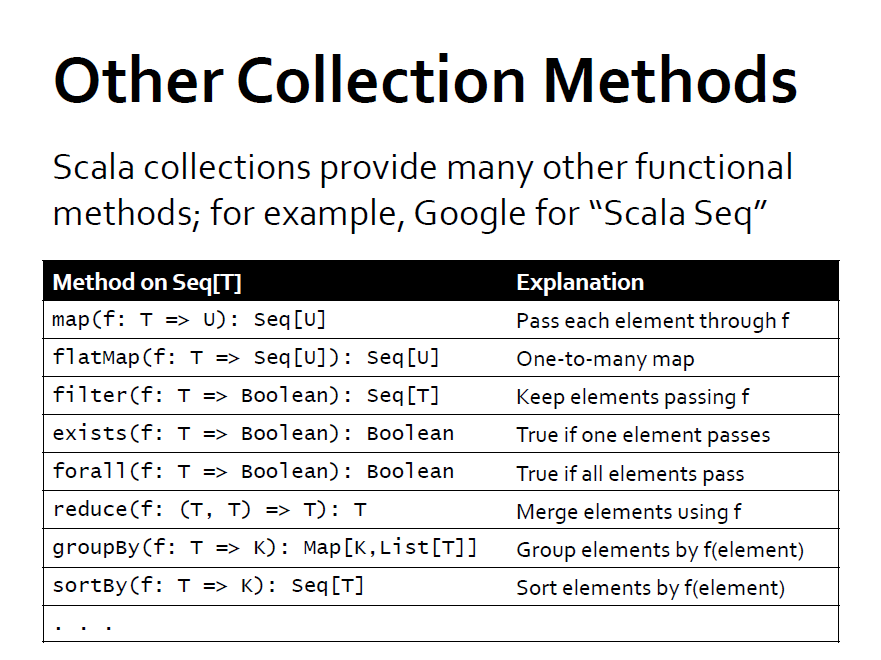
\includegraphics[height=\paperheight]{images/collectionsmethods.png}\hfil}\vfil}}%

\begin{frame}[plain]
\end{frame}
}

\begin{frame}[fragile]
  \frametitle{Spark specific methods}

  Some examples:

  \begin{itemize}
    \item collect: to apply all transformations and get their results
    \item cache: to save results for later use
    \item groupByKey: to group items by key
    \item reduceByKey\footnote{Prefer this to groupbykey+map+reduce. See the slides from our previous class for more information}: group and apply reduce in the same step
    \item<2-> keyBy: to creates [K,V] tuples by applying a function to each value
    \item<3-> ...
  \end{itemize}
\end{frame}

\begin{frame}
  \frametitle{Closer look at our demo}
  
  \center
{\huge  Now, I'll start using the terminal.}
\pause
{\huge Don't freak out}
\end{frame}

\begin{frame}[plain]
  \begin{tikzpicture}[remember picture,overlay]
    \node[at=(current page.center)] {
\href{https://www.youtube.com/watch?v=SOyZd3D65Z4}{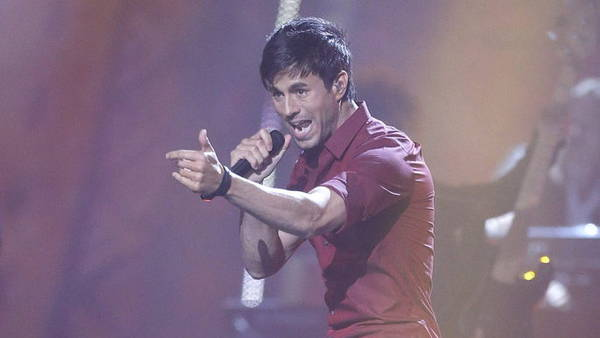
\includegraphics[width=\paperwidth]{images/enrique.jpg}}
            };
\end{tikzpicture}

\btVFill

\center
\Large Apologies in advance.
\vfill

\end{frame}

\section{Advanced Spark configuration}

\begin{frame}[fragile]
  \frametitle{Spark conf}
  \centering
\href{http://spark.apache.org/docs/latest/configuration.html}{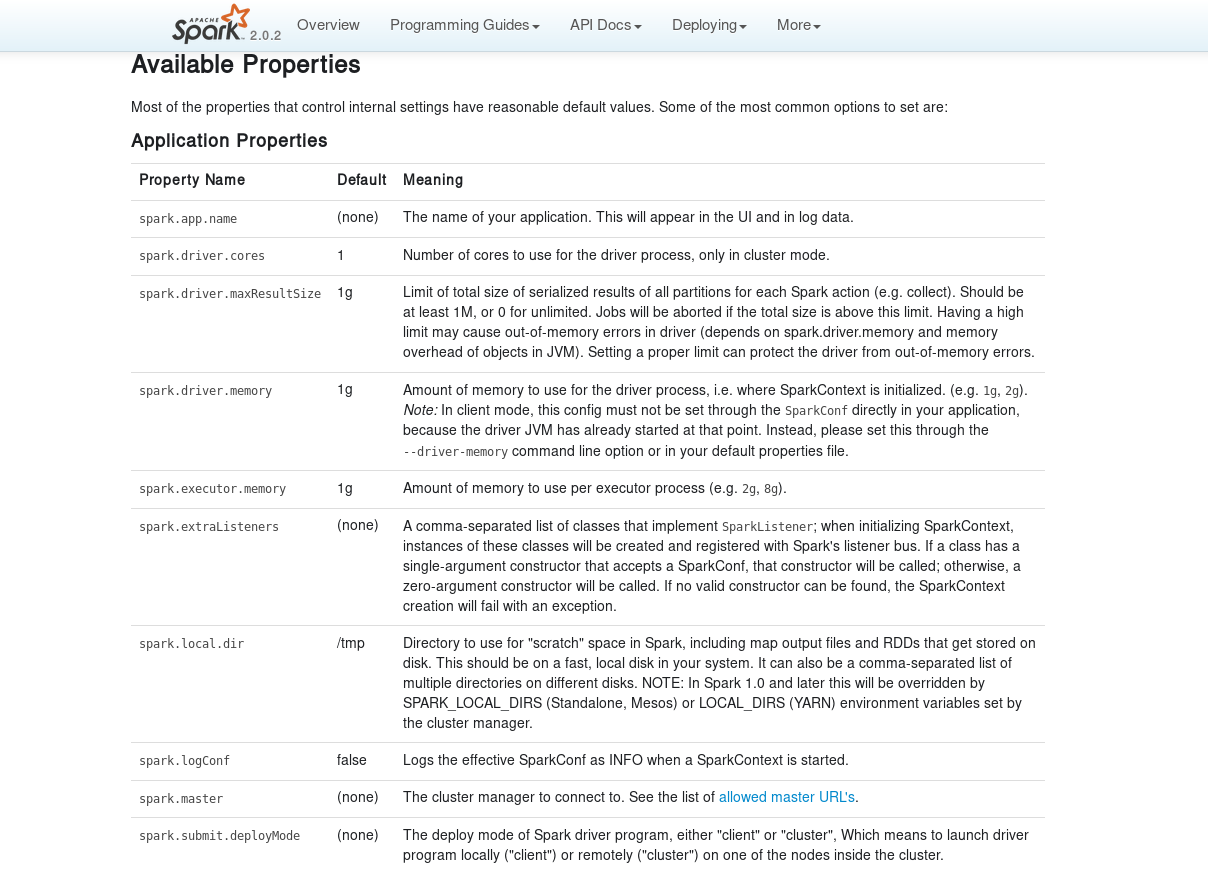
\includegraphics[width=\textwidth]{images/spark-conf.png}}

\end{frame}

\begin{frame}
  \begin{itemize}
    \item Application, Runtime, UI and RDD settings
    \item Highlights
      \begin{itemize}
        \item Master URL and Port
        \item CPU and memory per worker
        \item Parallelism: default partition size
      \end{itemize}
    
  \end{itemize}
\end{frame}


\section{Deploying a cluster with 20+ nodes}
\begin{frame}
  \frametitle{Our big data cluster}

  We will illustrate what we've already covered by deploying a cluster of more than 20 nodes.
  \pause
  
  Top of the line servers in Azure and Amazon.
  \pause

  Backed up by BlueMix's Spark infrastructure.
  
\end{frame}
\begin{frame}[plain]
  \begin{tikzpicture}[remember picture,overlay]
    \node[at=(current page.center)] {
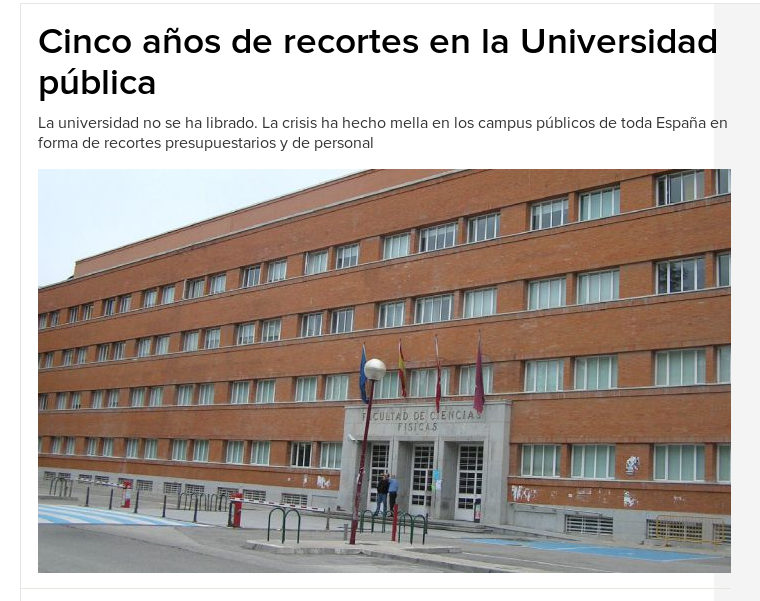
\includegraphics[width=\paperwidth]{images/recortes.png}
            };
\end{tikzpicture}

\end{frame}
\begin{frame}
  \frametitle{Our brain-powered cluster}

  \center
  {\huge This is embarrassing...}

  \pause
  
  {\huge We'll have to make do with our brains and paper.}

  \pause
  
  {\huge That's probably how Amazon Mechanical Turk was born.}

\end{frame}

\begin{frame}[fragile]
  \frametitle{Input}
  
We have a log of users that know or ask about a topic.
It looks like this:

\begin{verbatim}
  Alice knows Scala
  Bob asks about Scala
  Caroline asks about Java
  Don knows about Scala
   ...
\end{verbatim}

In other words, lines have this format:

\begin{verbatim}
  {student} {action} {topic}
\end{verbatim}

\end{frame}

\begin{frame}
  \frametitle{Your task}

  Answer the questions:
\begin{itemize}
  \item How many questions were asked about each topic?
    \pause
  \item How many times did each student ask about each topic?
    \pause
  \item (Harder) Is there any topic with questions that no other student knows about?
    \pause
  \item (Even harder) Pair students that know about a topic with students that don't

\end{itemize}
  
\end{frame}

\section{Different orchestrators}

\begin{frame}
  \frametitle{Spark architecture}
  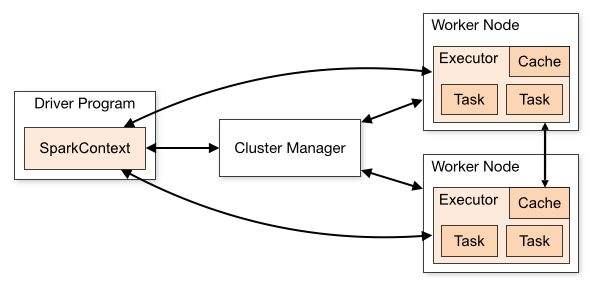
\includegraphics[width=\textwidth]{images/cluster-overview.png}
  \end{frame}

\begin{frame}
  \frametitle{Spark architecture}
  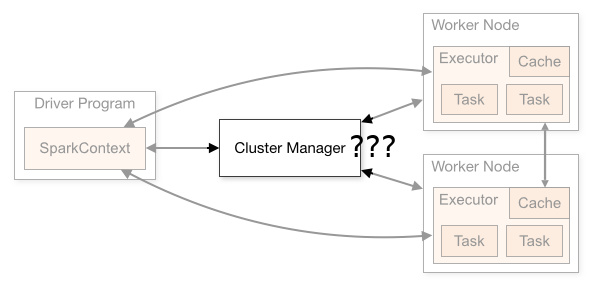
\includegraphics[width=\textwidth]{images/cluster-overview-question.png}
\end{frame}


\begin{frame}
  \frametitle{Cluster managers}
  \large Cluster managers (either Spark’s own standalone cluster manager, Mesos or YARN), which allocate resources across applications. Once connected, Spark acquires executors on nodes in the cluster, which are processes that run computations and store data for your application.
\end{frame}

\begin{frame}
  \frametitle{Mesos}
  \begin{tikzpicture}[remember picture,overlay]
    \node[at=(current page.center)] {
\href{https://github.com/apache/spark/tree/master/examples/src/main/scala/org/apache/spark/examples/}{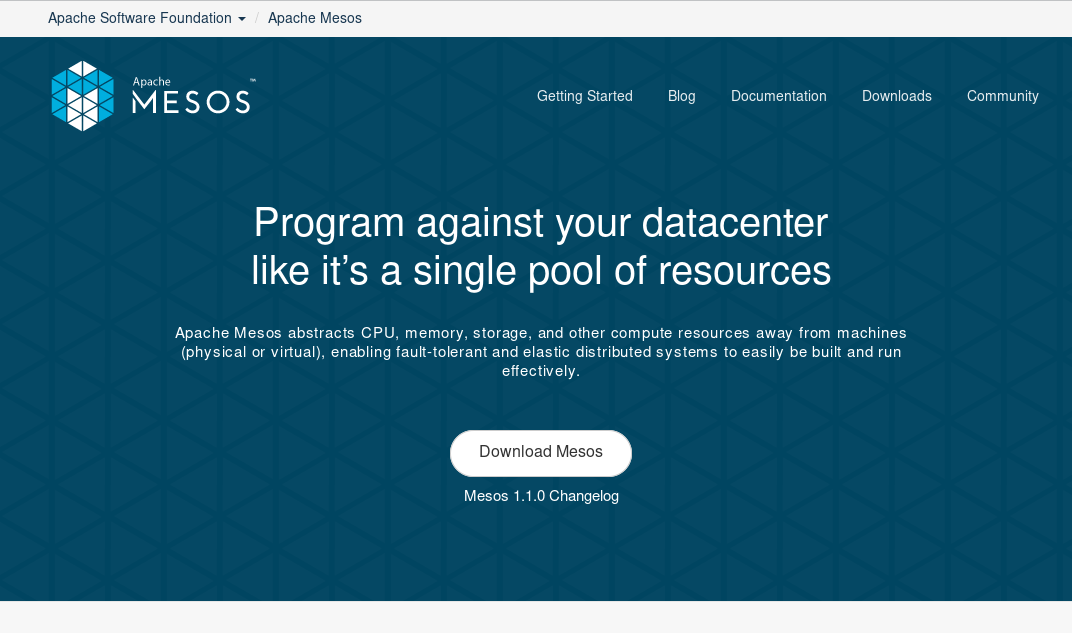
\includegraphics[width=\paperwidth]{images/mesosweb.png}}
            };
\end{tikzpicture}
\end{frame}

\begin{frame}
  \frametitle{Cluster managers}
  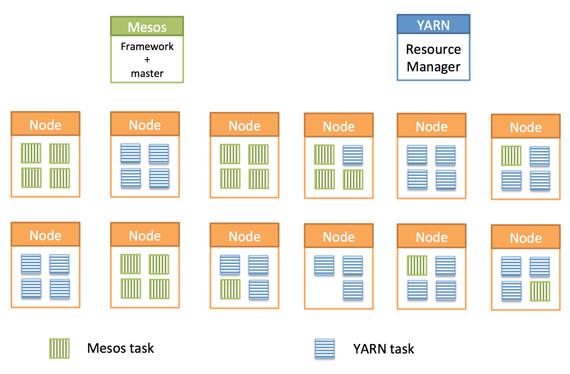
\includegraphics[width=\textwidth]{images/mesosyarn.png}
\end{frame}

\begin{frame}
  \frametitle{Spark architecture}
  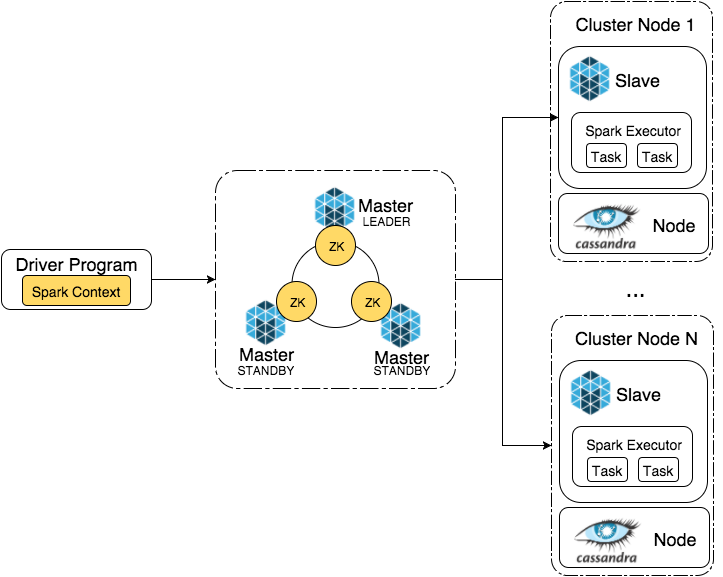
\includegraphics[height=.85\textheight]{images/mesos-spark.png}
\end{frame}

\begin{frame}
  \frametitle{Spark on mesos}
  \btVFill
  \center
  {\Large Once again, Spark has astoundingly good documentation}
  \btVFill

{\large  \href{http://spark.apache.org/docs/latest/running-on-mesos.html}{http://spark.apache.org/docs/latest/running-on-mesos.html}}
  \btVFill
\end{frame}


  
\section{Spark Ecosystem}

\begin{frame}
  \frametitle{Ecosystem}
  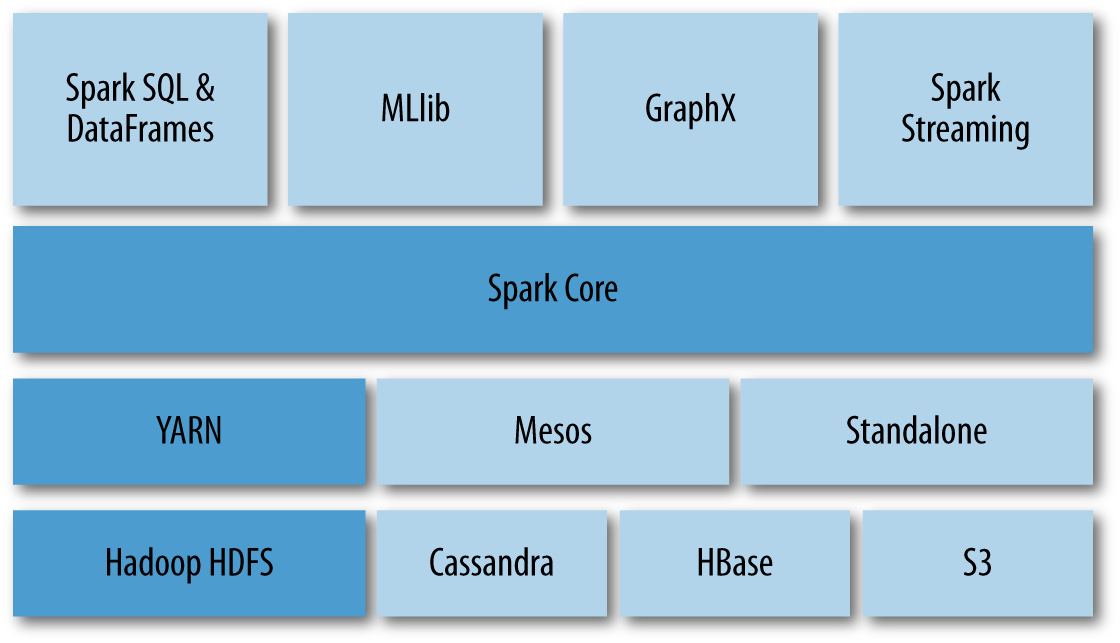
\includegraphics[width=\textwidth]{images/sparkecosystem.png}
\end{frame}


\begin{frame}[plain]
  \begin{tikzpicture}[remember picture,overlay]
    \node[at=(current page.center)] {
\href{https://github.com/apache/spark/tree/master/examples/src/main/scala/org/apache/spark/examples/}{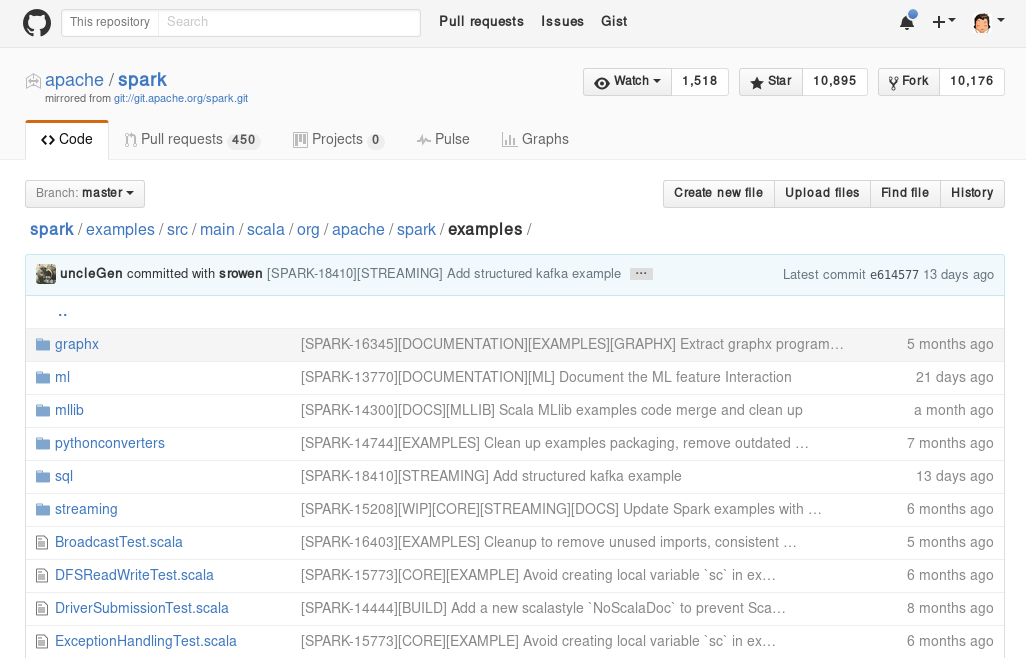
\includegraphics[width=\paperwidth]{images/examples.png}}
            };
\end{tikzpicture}

\end{frame}

\begin{frame}[fragile,allowframebreaks]
  \frametitle{Spark Streaming}
  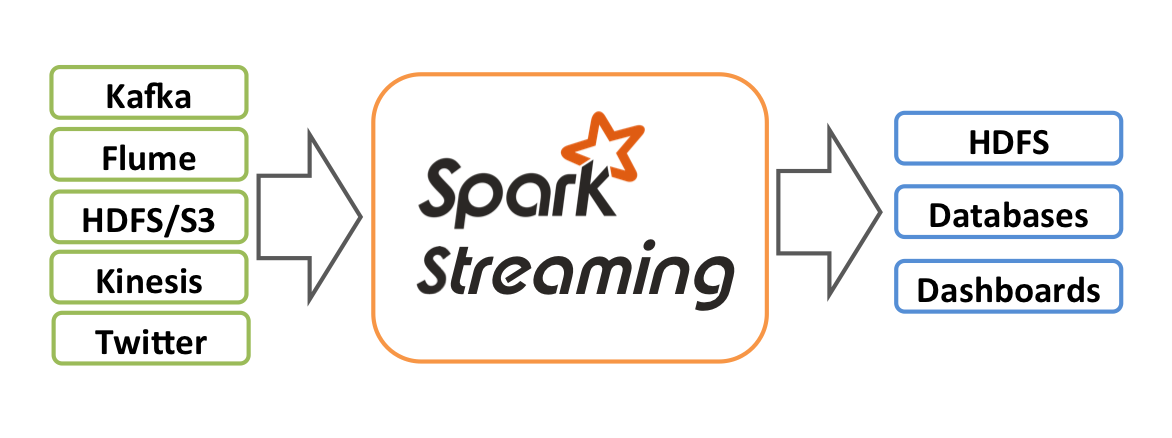
\includegraphics[width=\textwidth]{images/streaming-arch.png}

  \framebreak

  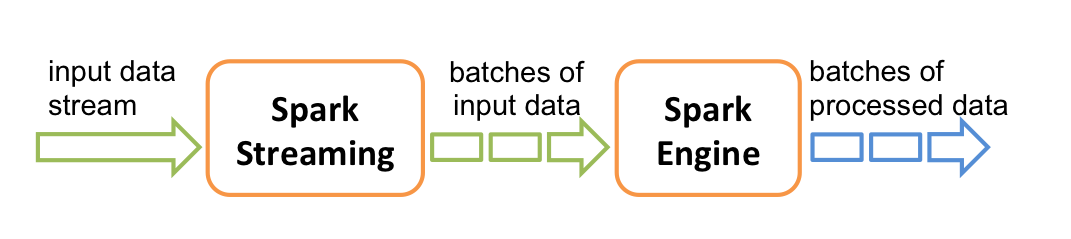
\includegraphics[width=\textwidth]{images/streaming-flow.png}
  
\end{frame}

\begin{frame}[fragile]
  \frametitle{Demo!}
  
We'll show a demo of a modified Spark Streaming task.

Here is a quick ``video'' of the demo: 
  {\Large \href{https://asciinema.org/a/6kp49z5m3hq9vja9r7x4rjq26}{https://asciinema.org/a/6kp49z5m3hq9vja9r7x4rjq26} }
  
All the code and instructions are available in our repository (in several branches):

{\Large \href{https://github.com/balkian/docker-spark}{https://github.com/balkian/docker-spark}}

\end{frame}

\section{Acknowledgements and useful links}

\begin{frame}
  \begin{itemize}
\item \href{http://spark.apache.org/docs/latest/programming-guide.html}{Spark programming guide}
\item \href{https://databricks.com/blog/2016/01/04/introducing-apache-spark-datasets.html}{Databricks introducing apache spark datasets}
\item \href{https://www.safaribooksonline.com/library/view/data-analytics-with/9781491913734/ch04.html}{Data Analytics with Hadoop: In-Memory Computing with Spark}
\item \href{https://trongkhoanguyenblog.wordpress.com/2014/11/27/understand-rdd-operations-transformations-and-actions/}{Understanding RDD operations, transformations and actions}
\item \href{http://spark.apache.org/docs/latest/streaming-programming-guide.html}{Spark Streaming programming guide}
  \end{itemize}
\end{frame}

\end{document}
